\documentclass[12pt]{article}
\usepackage[usenames,dvipsnames]{color}
\usepackage{listings}
\usepackage{graphicx}
\usepackage{fancyhdr}
\usepackage{framed}
\usepackage[T1]{fontenc}
\usepackage[toc,page]{appendix}
\usepackage[utf8]{inputenc}
\usepackage[brazil]{babel}
\usepackage{fancyvrb}
\usepackage[hmargin=2cm,vmargin=2cm]{geometry}
\usepackage{lastpage}
\usepackage{makeidx}
\pagestyle{fancy}

% cabecalho e rodapé
\setlength{\headheight}{120pt}
\setlength{\textheight}{550pt}
\renewcommand{\headrulewidth}{0pt}
\lhead{
\includegraphics[scale=0.03]{brasao.png}}
\rhead{
\includegraphics[scale=0.4]{logo-pnud.png}}
\cfoot{\textbf{\ProjectCode\ - Inovando a democracia participativa}}
\rfoot{\thepage}

\hyphenation{par-ti-ci-pa-ção}
\bibliographystyle{ieeetr}

% definições sobre o autor e o produto
\newcommand{\MyName}{Joenio Marques da Costa}
\newcommand{\MySurnameForename}{Costa, Joenio}
\newcommand{\SupervisorName}{Ricardo Augusto Poppi Martins}
\newcommand{\MyEmail}{joenio@colivre.coop.br}
\newcommand{\ContractNumber}{2013/000564}
\newcommand{\ContractYear}{2013}
\newcommand{\ProjectCode}{Projeto BRA/12/018}
\newcommand{\NomeSecretaria}{Secretaria Geral da Presidência da República}
\newcommand{\SiglaSecretaria}{SG/PR}
\newcommand{\ProductNumber}{06}
\newcommand{\ProductTitle}{Protocolos para federação de redes sociais}
\newcommand{\ProductSubtitle}{Proposta de federação entre o Participa.br e as
  redes Diaspora}
\newcommand{\ProductDescription}{"Documento com análise de protocolos,
  arquiteturas e sistemas de federação de conteúdos para ambientes de redes
  Sociais com estratégia de implantação considerando os sites parceiros e
  contendo propostas de códigos. Inclui especificações e códigos para conexão
  de contas e trocas de postagens do portal com redes sociais proprietárias."
}
\newcommand{\ProductValue}{R\$ 14.400,00 (quatorze mil e quatrocentos reais)}
\newcommand{\ObjetoContratacao}{"Construção dos códigos para comunidades e
  aplicativos do portal da participação social."
}
\newcommand{\DataEntrega}{25 Novembro de 2014}
\newcommand{\PalavrasChave}{federação, redes sociais, diaspora, descentralização}

% lista de abreviações
\makeindex

\begin{document}

\newgeometry{hmargin=3cm,vmargin=1.5cm}
\addtolength{\topmargin}{2.5cm}
\thispagestyle{empty}
{\color{MidnightBlue}

{\bf \LARGE Produto \ProductNumber\ -\ \ProductTitle}

\hrulefill

\vspace{1cm}

\begin{center}

{\bf \large Contrato n. \ContractNumber}

\vspace{1.5cm}

{\bf \large Objeto da contratação: \ObjetoContratacao}

\end{center}

\vspace{3.2cm}

Valor do produto: \ProductValue

\vspace{1.2cm}

Data de entrega: \DataEntrega

\vspace{1.2cm}

Nome do consultor: \MyName

\vspace{1.2cm}

Nome do supervisor: \SupervisorName

}

\vspace{2cm}

\begin{center}

\includegraphics[scale=0.04]{brasao.png} \\
{\bf \small \NomeSecretaria}
\end{center}

\restoregeometry
\newpage

\newgeometry{hmargin=3cm,vmargin=1.5cm}
\begin{center}
\thispagestyle{empty}
{\color{MidnightBlue}


\includegraphics[scale=0.9]{logo-pnud.png}

\vspace{4cm}

{\bf \large \ProjectCode\ - Desenvolvimento de Metodologias
de Articulação e Gestão de Políticas Públicas para Promoção da Democracia
Participativa}

\vspace{1.5cm}

{\bf \large Produto \ProductNumber\ -\ \ProductTitle}

\vspace{1.5cm}

\ProductSubtitle

\vspace{4cm}

\MyName

\vspace{2cm}

}


\includegraphics[scale=0.04]{brasao.png} \\
{\bf \small \NomeSecretaria}

\end{center}
\restoregeometry
\newpage

\newgeometry{hmargin=3cm,vmargin=1.5cm}
\addtolength{\topmargin}{2.5cm}
\thispagestyle{empty}
{\color{MidnightBlue}

{\bf \LARGE Produto \ProductNumber\ -\ \ProductTitle}

\hrulefill

\vspace{1cm}

\begin{center}

{\bf \large Contrato n. \ContractNumber}

\vspace{1.5cm}

{\bf \large Objeto da contratação: \ObjetoContratacao}

\end{center}

\vspace{3.2cm}

Valor do produto: \ProductValue

\vspace{1.2cm}

Data de entrega: \DataEntrega

\vspace{1.2cm}

Nome do consultor(a): \MyName

\vspace{1.2cm}

Nome do supervisor(a): \SupervisorName

}

\vspace{2cm}

\begin{center}

\includegraphics[scale=0.04]{brasao.png} \\
{\bf \small \NomeSecretaria}
\end{center}

\restoregeometry
\newpage

\newgeometry{hmargin=3cm,vmargin=1.5cm}
\addtolength{\topmargin}{5cm}
\thispagestyle{empty}

\begin{framed}

{\raggedright \MySurnameForename} \\

\ProductTitle: \ProductSubtitle\ / \ContractYear. \\

Total de folhas: \pageref{LastPage} \\

\vspace{1cm}

Supervisor: \SupervisorName \\

\SiglaSecretaria \\

\NomeSecretaria \\

Palavras-chave: \PalavrasChave. \\

\end{framed}

\vspace{3cm}

{\raggedright 
\includegraphics{licenca-cc-by-nc.png} \ Esta obra é licenciada sob
uma licença Creative Commons - Atribuição-NãoComercial. 4.0 Internacional.}

\restoregeometry
\newpage

\tableofcontents
\newpage

\begin{abstract}
Documento com análise de protocolos e ferramentas de federação para redes
sociais, proposta de implementação do protocolo Diaspora ao Noosfero,
integração entre Participa.br e redes Diaspora. \\

{\bf Palavras-chave:} \PalavrasChave.
\end{abstract}
\newpage

\section{Introdução}

Em consonância com os objetivos e cronograma previsto no âmbito do
projeto BRA/12/018:
\textbf{Desenvolvimento de Metodologias de Articulação e Gestão de
Políticas Públicas para Promoção da Democracia Participativa},
firmado entre a Secretaria-Geral da Presidência da República
(SG/PR) e o Programa das Nações Unidas para o Desenvolvimento (PNUD),
o presente documento apresenta \ProductDescription.

Essa proposta está configurada como produto \ProductNumber~da consultoria técnica
para especificação da construção dos códigos das metodologias de
organização da informação e interação participativa do portal de
participação social.

\section{O Participa.br}

O Participa.br é a Plataforma Federal da Participação Social. Trata-se de mais
um espaço para participação social no Brasil, escuta e diálogo entre o Governo
Federal e a Sociedade Civil. 

A plataforma, totalmente desenvolvida em software livre, tem como missão
desenvolver práticas inovadoras de participação via internet e oferta de
espaços de manifestação e debate para qualquer cidadão ou organização, com o
intuito de construir políticas públicas cada vez mais eficazes e efetivas.

O Participa.br é desenvolvido sob a plataforma para redes sociais Noosfero.

\section{O Noosfero}

O Noosfero\cite{noosfero} é uma plataforma web livre para redes sociais e de
economia solidária que possui as funcionalidades de Blog, e-Portfolios, CMS,
RSS, discussão temática, agenda de eventos e inteligência econômica
colaborativa num mesmo sistema! O Noosfero utiliza a linguagem de programação
Ruby com framework Rails e, portanto, suporta bancos de dados, PostgreSQL,
MySQL, SQLite entre outros.

Noosfero é um Software Livre e licenciado sob a GNU Affero General Public
License (AGPL), versão 3.

\section{Redes sociais federadas}

Federação é a combinação de multiplos sistemas de computação funcionando sobre
padrões de operação compatíveis entre sí. Ou seja, sistemas com estruturas
internas diferentes funcionando em conjunto de forma transparente
\cite{federacao}.

Em sistemas em rede, federação significa que os usuários conseguem enviar
mensagens de um sistema a outro através da rede, sendo estes sistemas
distintos entre sí mas seguindo padrões de comunicação previamente definidos.

Exemplos de sistemas federados são inúmeros, dentre eles podemos citar
sistemas de email, chats Jabber, chats IRC, dentre outros. A maneira de
funcionamento de cada sistema é única, para cada serviço há uma proposta
diferente, sistemas de email por exemplo seguem o protocolo de envios de
mensagens chamado SMTP\cite{smtp} que é o responsável por garantir federação
no envio das mensagens. Desta forma um sistema federado de troca de
mensagens é independente de plataforma, ou seja, usuários de um fornecedor de
email (exemplo GMail) podem interagir de forma transparente com usuários de
outros fornecedores (exemplo Hotmail).

Chats Jabber por outro lado se baseiam no protocolo chamado XMPP\cite{xmpp},
com ele usuários podem usar serviços distintos e conversarem entre sí de forma
transparente. Chats IRC são implementados com base no protocolo de mesmo nome
chamado IRC\cite{irc}, a Figura \ref{irc} traz um diagrama de rede IRC
descentralizada e federada
\footnote{fonte: https://pt.wikipedia.org/wiki/Ficheiro:Ircnetz-Schema.svg}.

\begin{figure}[h]
\center
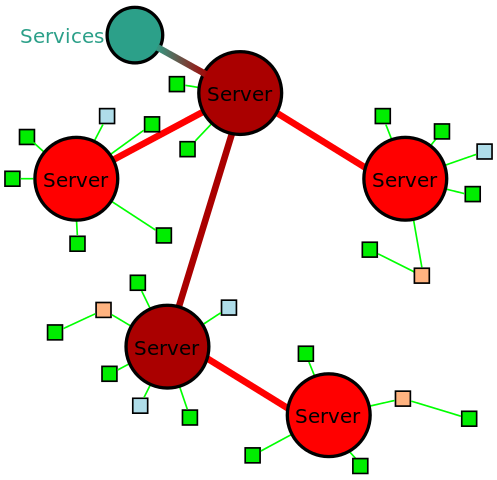
\includegraphics[scale=0.4]{Ircnetz-Schema.png}
\caption{Exemplo de rede federada IRC}
\label{irc}
\end{figure}

Todos estes exemplos tem servido como inspiração para o desenvolveimento de
protocolos de federação em redes sociais, as principais redes sociais modernas
não são federadas, além de serem extremamente centralizadas. Redes como
Facebook e Google Plus por exemplo obrigam os usuários a estarem cadastrados
em sua base da dados para poder interagir com seus usuários e comunidades.

Um movimento para quebrar este paradigma de redes sociais extremamente
isoladas começou a surgir através do termo {\it redes sociais virtuais
federadas}, o termo {\it federada} foi usado em detrimento do termo {\it
aberta} para não causar confusão pois ela é mais específica e estabelece
claramente o que se pretende: criar redes sociais que se interconectem entre
sí de forma transparente. Este movimento foi iniciado em 2010 a partir de um
evento chamado {\it Federated Social Web Conference}\cite{aurelio}.

\section{Protocolos para federação de redes sociais}

Inúmeras iniciativas e propostas tem surgido para solucionar o isolamento das
redes sociais e promover interoperabilidade e descentralização, alguns
dos protocolos mais populares e comumente referenciados são listados a seguir.

\subsection{Activity Streams}

É uma especificação de formato aberto para um protocolo de {\it streaming} de
atividades, com foco em criar um consórcio entre aplicações e serviços
web, um {\it streaming} de atividades é algo similar a linha do tempo do
Facebook.

A maior implementação do protocolo é o Stream Framework\cite{stream}, uma
biblioteca em Python para construção de fonte de notícias usando Cassandra ou
Redis.

A especificação do protocolo\cite{streams} basicamente define um formato comum
para transmitir informações do tipo: "Geraldino postou uma foto em seu álbum"
ou "João compartilhou um vídeo".

\begin{itemize}
  \item http://en.wikipedia.org/wiki/Activity\_Streams\_(format)
\end{itemize}

\subsection{Diaspora's Federation Protocol}

O protocolo Diaspora descreve como deve ocorrer a comunicação entre servidores
Diaspora. O compartilhamento através deste protocolo é assimétrica, ou seja,
em um relacionamento um usuário inicia compartilhamento com alguém, mesmo que
esse alguém nao deseje compartilhar algo. Desta forma um usuário pode
compartilhar tudo com um outro certo usuário que não deseje compartilhar nada
com ele. O envio de postagens é feito através do protocolo Salmon.

\begin{itemize}
  \item https://wiki.diasporafoundation.org/Federation\_Protocol\_Overview
\end{itemize}

\subsection{FOAF}

FOAF é uma ontologia para descrição de pessoas, suas ativiades e seus
relacionamentos com foco na fácil leitura por máquinas. Qualquer um pode usar
FOAF para descrever a sí mesmo, com ele é possível descrever redes sociais sem
necessidade de um banco de dados centralizado.

É um vocabulário descritivo expressado em RDF e OWL, computadores podem
usar os perfis FOAF para encontrar, por exemplo, todas as pessoas vivendo na
Europa, ou para listar todas as pessoas que são amigas de alguém. Cada perfil
tem um identificador único usado para definir estas relações.

O projeto foi iniciado em 2000 e pode ser considerado a primeira aplicação da
Web Semantica, que combina tecnologia RDF com conceitos da 'Web Social'.

\begin{itemize}
  \item http://en.wikipedia.org/wiki/FOAF\_(ontology)
\end{itemize}

\subsection{Google Wave Federation Protocol}

Um protocolo aberto descrito como uma extensão do protocolo XMPP\cite{xmpp},
usado no projeto chamado {\it Apache Wave}\cite{wave}, projetado para
comunicação em tempo real através de servidores trabalhando de forma
cooperativa.

O protocolo é fortemente baseado nos protocolos de email e as funcionalidades
implementadas são formetemte inspiradas nestes sistemas.

\begin{itemize}
  \item http://en.wikipedia.org/wiki/Google\_Wave\_Federation\_Protocol
\end{itemize}

\subsection{OStatus}

OStatus é um padrão aberto para compartilhamento de atualizações, faz
referencias a protocolos abertos como Atom, Activity Streams, PubSubHubbub,
Salmon e Webfinger. Através dele são criados pontos de troca, roteamento de
mensagens e atualizações de status entre usuários em tempo real.

O OStatus foi inicialmente implementado no StatusNet e posterioemente em
MiniMe, ambos projetos de microblogs. Em janeiro de 2012 o W3C adotou e passou a
manter o OStatus. Hoje é implementado na plataforma GNU Social.

\begin{itemize}
  \item http://en.wikipedia.org/wiki/OStatus
\end{itemize}

\subsection{OpenSocial}

OpenSocial é uma especificação pública que define um componente de hospedagem
e um conjunto de APIs para aplicações web de redes sociais, foi desenvolvido
em conjunto pelo Google, MySpace e outras redes sociais. A OpenSocial
Foundation suporta várias outras tecnologias Web como OAuth, Activity Streams
e Portable Contacts.

Foi lançado em Novembro de 2007, as aplicações que implementam o OpenSocial
podem interoperar com qualquer outra rede social que tenha suporte a ele.

\begin{itemize}
  \item http://en.wikipedia.org/wiki/OpenSocial
\end{itemize}

\subsection{PubSubHubbub}

PubSubHubbub é um protocolo aberto para comunicação distribuída de publicação
e inscrição, inicialmente projetado para estender os protocolos Atom e RSS,
pode ser aplicado para qualquer tipo de dado (texto, imagens,
audio, vídeos) desde que estejam disponívels via HTTP.

O principal objetivo é prover notificações de mudanças em tempo real. É
utilizado para publicar conteúdo de uma única vez em diversos sites. Entre os
sites suportados por este protocolo podemos citar: blogger.com, wordpress.com,
CNN, Fox News, diaspora*, entre outros.

\begin{itemize}
  \item http://en.wikipedia.org/wiki/PubSubHubbub
\end{itemize}

\subsection{Pump.io}

Pump.io é um motor de {\it streaming} de atividades de propósito geral que
pode ser usado como protocolo de rede social federada. Seu criador afirma que
"ele faz o que a maioria das pessoas realmente precisam de uma rede social", é
uma evolução do StatusNet e hoje encontra-se em produção no serviço {\it
Identi.ca}.

Apesar de ter sido inicialmente baseado no StatusNet, que oferece serviço
similar o Twitter, o pump.io oferece recursos muito mais gerais de rede
social, e tem sido adotado por outros tipos de aplicação, como o
MediaGoblin\footnote{http://www.mediagoblin.org} por exemplo.

\begin{itemize}
  \item http://en.wikipedia.org/wiki/Pump.io
\end{itemize}

\subsection{Salmon}

O protocolo Salmon é um protocolo para troca de mensagens sob HTTP projetado
para descentralizar comentários e anotações feitas em artigos e posts de
blogs. Permite discussões através de comentários vindos de diversos pontos
distintos através de um "agregador" que está inscrito e obtendo o conteúdo
destas fontes. De forma simples, um artigo apresentado em 3 sites distintos: A
(fonte original), B e C podem receber comentários vindos de usuários de
qualquer um dos 3 sites, estes comentários são sincronizados entre os 3
e todos os usuários podem interagir de forma transparente através deles.

Redes sociais federadas como StatusNet e Diaspora usam Salmon para coordenar
discussão entre usuários de diferentes servidores. Um usuário de um servidor
pode publicar um artigo que será disseminado para outros usuários de outras
redes via Salmon, que em contrapartida podem comentar de volta de maneira
transparente.

\begin{itemize}
  \item http://en.wikipedia.org/wiki/Salmon\_(protocol)
\end{itemize}

\subsection{Tent}

Tent é um protocolo para redes sociais abertas e descentralizadas.  Qualquer
um pode executar um servidor Tent, ou escrever um aplicativo alternativo que
use o seu protocolo. Usuários podem ter o controle sobre o conteudo e seus
relacionamentos alterando ou movendo-se entre os servidores. Tent suporta uma
lista extensiva de tipos de dados, e possui capacidade de ser extendido com
novos tipos de interação.

\begin{itemize}
  \item http://en.wikipedia.org/wiki/Tent\_(protocol)
\end{itemize}

\subsection{WebFinger}

Protocolo especificado pelo IETF permite descobrir informações sobre pessoas e
objetos identificados por URIs únicas. Informações sobre uma pessoa pode ser
descoberta através de uma requisição "acct:", contendo um endereço similar a
um email no formato "usuario@servidor".

É usado por redes como StatusNet e Diaspora para descobrir usuário em nós
federados e "pods", ou em protocolos de armazenamento remoto como ownCloud por
exemplo. Foi derivado historicamente do protocolo Finger, mas possui muitas
diferenças por ser projetado sob o HTTP.

\begin{itemize}
  \item http://en.wikipedia.org/wiki/WebFinger
\end{itemize}

\section{Ferramentas de redes sociais federadas}

Estes protocolos isoladamente não fornecem a solução para descentralizar as
redes e promover federação entre elas, é preciso ter ferramentas implementando
tais protocolos. Cada protocolo resolve um problema específico, a combinação
deles em uma implementação resulta num produto abrangente que resolve o
problema de centralização das redes. Nas próximas sessões serão apresentadas
algumas ferramentas de rede social federada.

\subsection{Diaspora}

Diaspora é projetado para atacar problemas relacionados a privacidade em redes
sociais centralizadas permitindo aos usuários subirem seu próprio servidor
(chamado "pod") e desta forma hospedar seu próprio conteúdo. Estes "pods" podem
interagir entre sí para compartilhar atualização de status, fotos e outros tipos de
conteúdo.

Uma parte central do software Diaspora é que ele deve funcionar como um
"agregador social", permitindo posts serem facilmente importados e exportados
entre os vários "pods", além de proporcionar interação com redes fechadas como
Facebook, Tumblr e Twitter. A ideia é quebrar as barreiras legais para juntar as
diversas redes sociais, quanto mais pessoas entrarem, menos força e poder as
redes sociais fechadas e proprietárias terão, garantindo desta forma mais
liberdade para os usuários.

O software Diaspora implementa um protocolo de mesmo nome, além do WebFinger,
Salmon, Activity Stream e o micro-formato h-card.

\begin{itemize}
  \item http://en.wikipedia.org/wiki/Diaspora\_(software)
\end{itemize}

\subsection{Friendica}

Friendica é um software livre que implementa uma rede social distribuída,
possui grande preocupação com privacidade e facilidade na instalação de
servidores. Tem como missão integrar de forma federada tantas redes quanto
possível, atualmente integra com: Facebook, Twitter, Diaspora, GNU social,
App.net, Pump.io, WordPress, Livejournal, Tumblr e Posterous. Em novembro de
2014, o diretório global de usuários do Friendica contabiliza 10 mil
registros, número de usuários que decidiram publicar seus perfis no diretório
público global.

\begin{itemize}
  \item http://en.wikipedia.org/wiki/Friendica
\end{itemize}

\subsection{StatusNet / GNU Social}

GNU Social, chamado no passado de StatusNet, é um servidor de microblog livre
escrito em PHP que implementa o padrão OStatus para interoperação entre
instalações. Enquanto oferece funcionalidade similar ao Twitter, StatusNet
tenta prover o potencial para promover comunicação entre comunidades de
microblog abertas e distribuídas.

É baseado no protocolo OStatus, mas também suporta Salmon e OpenID.

\begin{itemize}
  \item http://en.wikipedia.org/wiki/GNU\_social
\end{itemize}

\section{Federação entre o Participa.br e Diaspora}

Dentre os softwares citados anteriormente o Diaspora foi escolhido como um
plano piloto para ser integrado ao Participa.br, nas sessões que seguem será
descrito como o Diaspora funciona em detalhes tecnicos, quais os passos para
integrar o Participa.br a ele, e como integrar outras redes que também usem
o Noosfero entre sí.

\subsection{Diaspora em detalhes}

% * pesquisa o protocolo do diaspora
% * detalhes sobre este protocolo
% * nível de maturidade, aceitação e adoção

O Diaspora é tanto uma implamentação de uma ferramenta de rede social, quanto
uma especificação de protocolo para federação. A implementação suporta as
seguintes funcionalidades:

\begin{itemize}
  \item Status messages
  \item Blogging
  \item Photo sharing
  \item Privacy enhanced
\end{itemize}

É implementado em Ruby on Rails, licenciado sob a licença AGPL e implementa os
seguintes protocolos:

\begin{itemize}
  \item Salmon
  \item WebFinger
  \item Activity Stream
  \item h-card
\end{itemize}

Além do Ruby on Rails depende de HAML, SASS, Backbone.js e Handlebars.js, o
seu banco de dados possui a seguinte estrutuda:

\begin{itemize}
  \item User - Representação de um usuário no banco de dados
  \item Person - A representação de um usuário para o mundo exterior
  \item Contact - Define relações entre pessoas
  \item Request - Requisição de amizade entre pessoas
  \item Aspect - Uma lista de pessoas e postagens
  \item Post - Uma postagem associada a uma pessoa
\end{itemize}

O workflow ao postar algo no Diaspora segue os seguintes passos:

\begin{itemize}
  \item Quando um usuário posta algo, o Diaspora posta em um ou vários Aspect
  \item Assumindo que o post é válido, é armazenado no banco de dados em {\it raw\_visible\_posts}
  \item O HTML deste post é renderizado no servidor e enviado para o usuário via WebSocket\cite{websocket}
  \item O post é então serializado para XML e assinado em um envelope Salmon
\end{itemize}

\begin{framed}
\begin{lstlisting}[caption=Exemplo envio de mensagem e como o Diaspora serializa em XML]
  post.to_diaspora_xml
      def push_to_people(post, people)
        salmon = salmon(post)
        people.each{|person|
          xml = salmon.xml_for person
          push_to_person( person, xml)
        }
      end
  
  Salmon::SalmonSlap.create
      def self.create(user, activity)
        salmon = self.new
        salmon.author = user.person
        aes_key_hash = user.person.gen_aes_key
        salmon.aes_key = aes_key_hash['key']
        salmon.iv      = aes_key_hash['iv']
        salmon.magic_sig = MagicSigEnvelope.create(user,
          user.person.aes_encrypt(activity, aes_key_hash))
        salmon
      end
\end{lstlisting}
\end{framed}

Ao receber um post o fluxo é o seguinte:

\begin{itemize}
  \item O usuário recebe um Salmon, desencripta os cabeçalhos
  \item Se a assinatura do Salmon é válida ele é desempacotado e salvo no banco de dados
  \item Este post é armazenado entre os posts visiveis
\end{itemize}

De forma geral este é o funcionamento do Diaspora, mais detalhes sobre seu
funcionamento e implementação deve ser consultado na wiki do projeto ou
diretamente em seu código fonte:

\begin{itemize}
  \item http://wiki.diasporafoundation.org
  \item http://github.com/diaspora/diaspora
\end{itemize}

\subsection{Integração entre Participa.br e o Diaspora}

Para possibilitar integração entre o Participa.br e o Diaspora é preciso
implementar no Noosfero, software por trás do Participa.br, suporte aos
protocolos utilizados no Diaspora, ou seja: Salmon, Activity
Stream, WebFinger, h-card e o proprio protocolo Diaspora. Após esta
implementação tanto o Participa.br, quanto outras redes utilizando o Noosfero
poderão se comunicar com servidores Diaspora, um exemplo desta comunicação
pode ser visto no diagrama representado na Figura \ref{ecosistema}.

\begin{figure}[h]
\center
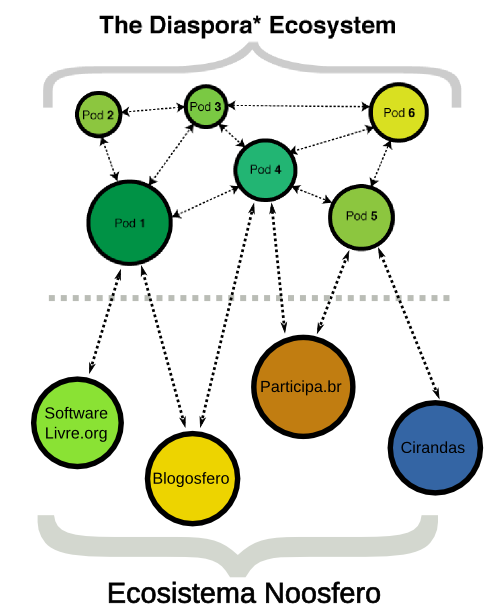
\includegraphics[scale=0.4]{ecosistema-noosfero-diaspora.png}
\caption{Diagrama sobre integração entre o ecosistema Noosfero e Diaspora}
\label{ecosistema}
\end{figure}

\subsubsection{WebFinger e Noosfero}

O WebFinger é um protocolo para descoberta de informações sobre pessoas e
objetos identificados por URIs únicas. Ele é o primeiro passo para ter
interação real com o Diaspora e outras redes sociais federadas.

O Noosfero não tem suporte a tal protocolo, mas houve uma iniciativa pessoal
de um dos desenvolvedores do Noosfero em documentar algo sobre ele e iniciar
uma implementação:

\begin{itemize}
  \item Issue sobre WebFinger no tracker do Noosfero: \\
    http://noosfero.org/Development/ActionItem1573
  \item Branch no Git com a implementação parcial para WebFinger: \\
    https://gitlab.com/aurium/noosfero/commits/init-federation
\end{itemize}

É preciso evoluir esta implementação para ter suporte completo ao protocolo
WebFinger de forma que os usuários da rede possam ser consultados através de
suas URIs pelos outros "pods", os usuários do Participa.br deverão ser
identificados através de endereços no seguinte formato:

\begin{itemize}
  \item usuario@participa.br
\end{itemize}

Um usuário fictício chamado "Joao", por exemplo, será identificado através da
seguinte URI WebFinger:

\begin{itemize}
  \item joao@participa.br
\end{itemize}

A partir desta URI um "pod" Diaspora poderá consultar e descobrir informações
sobre "Joao" a partir de uma requisição do tipo "acct:joao@participa.br". Esta
requisição deve retornar algo do tipo:

\begin{framed}
\begin{lstlisting}[caption=Exemplo resposta a consulta WebFinger]
HTTP/1.1 200 OK
Access-Control-Allow-Origin: *
Content-Type: application/jrd+json
{
  "subject" : "acct:joao@participa.br",
  "aliases" :
  [
    "https://participa.br/joao"
  ],
  "properties" :
  {
      "http://participa.br/ns/role" : "member"
  },
  "links" :
  [
    {
      "rel" : "http://webfinger.example/rel/profile-page",
      "href" : "https://participa.br/profile/joao"
    },
    {
      "rel" : "http://webfinger.example/rel/businesscard",
      "href" : "https://participa.br/profile/joao/joao.vcf"
    }
  ]
}
\end{lstlisting}
\end{framed}

De posse destas informações será possível ter conhecimento sobre os recursos
deste usuário: onde está seu perfil, onde encontrar seu avatar, seu h-card, e
demais informações. Possibilitando aplicações externas obter informações sobre
os usuários da rede.

\subsubsection{Salmon e Noosfero}

O protocolo Salmon é um protocolo para troca de mensagens sob HTTP projetado
para descentralizar comentários e anotações feitas em artigos, como posts de
blogs, notícias, imagens, vídeos, eventos, entre outros.

O Noosfero não tem qualquer implementação ou iniciativa de implementar Salmon,
este protocolo é necessário para que o Noosfero ao menos se torne um {\it
aggregator} Salmon, ou seja quem lê uma feed de dados Salmon.

O Noosfero deve ser capaz de ser um "aggregator" para ler um feed Salmon
localizado no lado Diaspora. Quando um usuário do lado do Noosfero deixa um
comentário neste feed, o Noosfero deve armazenar o comentário de forma usual,
e então realizar um requisição POST\cite{salmon} seguindo a versão Salmon da
fonte do feed.

Esta requisição post tem o seguinte formato:

\begin{framed}
\begin{lstlisting}[caption=Exemplo requisição POST Salmon]
POST /salmon-endpoint HTTP/1.1
Host: example.org
Content-Type: application/atom+xml

<?xml version='1.0' encoding='UTF-8'?>
<me:env xmlns:me="http://salmon-protocol.org/ns/magic-env">
    <me:data type='application/atom+xml'>
    PD94bWwgdmVyc2lvbj0nMS4wJyBlbmNvZGluZz0nVVRGLTgnPz4KPGVudHJ5IH
    dodHRwOi8vd3d3LnczLm9yZy8yMDA1L0F0b20nPgogIDxpZD50YWc6ZXhhbXBs
    MjAwOTpjbXQtMC40NDc3NTcxODwvaWQ-ICAKICA8YXV0aG9yPjxuYW1lPnRlc3
    BsZS5jb208L25hbWUPHVyaT5hY2N0OmpwYW56ZXJAZ29vZ2xlLmNvbTwvdXJpP
    G9yPgogIDx0aHI6aW4tcmVwbHktdG8geG1sbnM6dGhyPSdodHRwOi8vcHVybC5
    ZD4KPC9lbnRyeT4KICAgIA
    </me:data>
    <me:encoding>base64url</me: <me:alg>RSA-SHA256</me:alg>
    <me:sig>
    EvGSD2vi8qYcveHnb-rrlok07qnCXjn8YSeCDDXlbhILSabgvNsPpbe76up8w63i2f
    WHvLKJzeGLKfyHg8ZomQ
    </me:sig>
</me:env>
\end{lstlisting}
\end{framed}

Com o suporte ao Salmon o Noosfero será capaz de ao receber comentários em
posts de blogs, notícias e afins, compartilhar estes comentários com usuários
em redes Diaspora.

Para concretizar esta implementação será preciso avaliar as seguintes
biblitecas abaixo, elas são implementações do protocolo Salmon para Ruby, uma
entre elas deve ser implementada no Noosfero.

\begin{itemize}
  \item https://github.com/sporkmonger/salmon
  \item https://github.com/hotsh/ostatus
\end{itemize}

\subsubsection{Activity Stream e Noosfero}

Activity Streams é uma especificação de formato aberto para um protocolo de
{\it streaming} de atividades, com ele é possível criar consórcio entre
aplicações e serviços web. {\it Streaming} de atividades é algo similar a
linha do tempo do Facebook. Com ele é possível ter um padrão comum de
comunicação para troca de dados relacionados às atividades dos usuários.

O Noosfero não tem suporte a este protocolo e precisa ser implementado
conformo a especificação do mesmo, basicamente uma atividade consiste de um
ator, um verbo, um objeto e um alvo. Ele conta a história de uma pessoa
realizando ações em um objeto, exemplos\cite{streams}:

\begin{itemize}
  \item "Geraldine postou uma foto em seu album"
  \item "João compartilhou um video"
\end{itemize}

\begin{framed}
\begin{lstlisting}[caption=Exemplo simples de atividade Activity Stream JSON serializada]
{
  "published": "2011-02-10T15:04:55Z",
  "actor": {
    "url": "http://participa.br/joao",
    "objectType" : "person",
    "id": "tag:participa.br,2011:joao",
    "image": {
      "url": "http://participa.br/profile/joao/image",
      "width": 250,
      "height": 250
    },
    "displayName": "Joao Silva"
  },
  "verb": "post",
  "object" : {
    "url": "http://participa.br/blog/2011/02/entry",
    "id": "tag:participa.br,2011:abc123/xyz"
  },
  "target" : {
    "url": "http://participa.br/blog/",
    "objectType": "blog",
    "id": "tag:participa.br,2011:abc123",
    "displayName": "Joao's Blog"
  }
}
\end{lstlisting}
\end{framed}

O Noosfero implementa {\it streaming} de atividades internamento de forma
nativa através do plugin Rails localizado em:

\begin{itemize}
  \item vendor/plugins/action\_tracker
\end{itemize}

Esta implementação não suporta nenhum tipo de integração com o protocolo
Activity Stream ou qualquer outro tipo de protocolo para federação, o inclusão
do suporte a este protocolo deve ser implementado nos arquivos citados acima,
ou seja, o plugin Rails {\it action\_tracker} deve ser adaptado para suportar
federação através do protocolo Activity Stream.

Exemplos de implementação podem ser consultados como forma de inspiração em:

\begin{itemize}
  \item https://github.com/GetStream/stream-rails
  \item https://github.com/GetStream/stream-ruby
\end{itemize}

\subsubsection{Diaspora e Noosfero}

O protocolo Diaspora descreve como deve ocorrer a comunicação entre servidores
Diaspora, com ele as seguintes acões podem ser tomadas:

\begin{itemize}
  \item Compartilhar notificações
  \item Des-compartilhar notificações
  \item Atualização de status
  \item Comentários em atualização de status
  \item Curtir em atualizações de status
\end{itemize}

Paralelo a cada uma dessas ações existem algumas diretivas importantes a serem
consideradas, e que devem ficar em mente durante a implementação. Uma delas é
a noção de usuários locais e usuarios remotos, alguns usuários estão no
servidor "pod" local outros estão em um "pod" remoto. Eles são tratados de
forma diferente pelo protocolo. Outra diretiva é que algumas vezes atividades
afetam tanto pessoas no "pod" local quanto em "pods" remotos, nestas situações
o Diaspora deve entregar primeiro localmente, em seguida tratar da entrega
remota.

Com isto em mente e de olho na especificação do protocolo o Noosfero deve ser
extendido para adicionar tal protocolo, idealmente isto deve ser feito no
formato de um plugin Noosfero, nos mesmos moldes do plugin OAuth mencionado em
mais detalhes na sessão \ref{sessao-oauth}. Segue referências detalhadas
sobre o protocolo Diaspora:

\begin{itemize}
  \item https://wiki.diasporafoundation.org/Federation\_protocol\_overview
  \item https://wiki.diasporafoundation.org/Diaspora\_message\_passing
  \item https://wiki.diasporafoundation.org/Federation\_message\_semantics
\end{itemize}

Segue alguns exemplos de mensagens trocada entre "pods".

\begin{framed}
\begin{lstlisting}[caption=Exemplo de notificação de compartilhamento]
<XML>
  <post>
    <request>
      <sender_handle>joao@participa.br</sender_handle>
      <recipient_handle>maria@softwarelivre.org</sender_handle>
    </request>
  </post>
</XML>
\end{lstlisting}
\end{framed}

\begin{framed}
\begin{lstlisting}[caption=Exemplo de atualização de status]
<XML>
  <post>
    <status_message>
      <raw_message>((status message))</raw_message>
      <guid>((guid))</guid>
      <diaspora_handle>joao@participa.br</diaspora_handle>
      <public>false</public>
      <created_at>2011-07-20 01:36:07 UTC</created_at>
    </status_message>
  </post>
</XML>
\end{lstlisting}
\end{framed}

\begin{framed}
\begin{lstlisting}[caption=Exemplo de comentário em uma atualização de status]
<XML>
  <post>
    <comment>
      <guid>((guid))</guid>
      <parent_guid>((guid))</parent_guid>
      <author_signature>((base64-encoded data))</author_signature>
      <text>Eu estou aqui!</text>
      <diaspora_handle>joao@participa.br</diaspora_handle>
    </comment>
  </post>
</XML>
\end{lstlisting}
\end{framed}

\subsubsection{h-card e Noosfero}

h-card é um formato aberto para publicar pessoas e organizações na Web. Ele é
um entre muitos microformatos voltados para incluir dados em HTML/HTML5.
h-card é uma atualização em cima do hCard.

\begin{framed}
\begin{lstlisting}[caption=Exemplo de h-card]
<p class="h-card">
  <img class="u-photo" src="http://example.org/photo.png" alt="" />
  <a class="p-name u-url" href="http://example.org">Joe Bloggs</a>
  <a class="u-email" href="mailto:joebloggs@example.com">
    joebloggs@example.com
  </a>, 
  <span class="p-street-address">17 Austerstrti</span>
  <span class="p-locality">Reykjavik</span>
  <span class="p-country-name">Iceland</span>
</p>
\end{lstlisting}
\end{framed}

Será preciso implementar h-card para os perfils de usuários do Noosfero,
apesar do Noosfero não suportar h-card diretamente, há algum suporte para
vCards, uma especificação mais ampla onde o h-card se insere, os arquivos do
Noosfero que precisam ser verificados e extendidos para adicionar suporte a
h-card são:

\begin{itemize}
  \item app/views/blocks/profile\_info.html.erb
  \item app/views/blocks/profile\_image.html.erb
  \item app/helpers/application\_helper.rb
  \item app/views/comment/\_comment\_actions.html.erb
\end{itemize}

O h-card é o formato onde os dados de cada perfil de usuário será publicado
para que outras redes leiam e obtenham informações sobre o usuário.

\subsection{Integração entre redes Noosfero}
\label{sessao-oauth}

\begin{figure}[h!]
\center
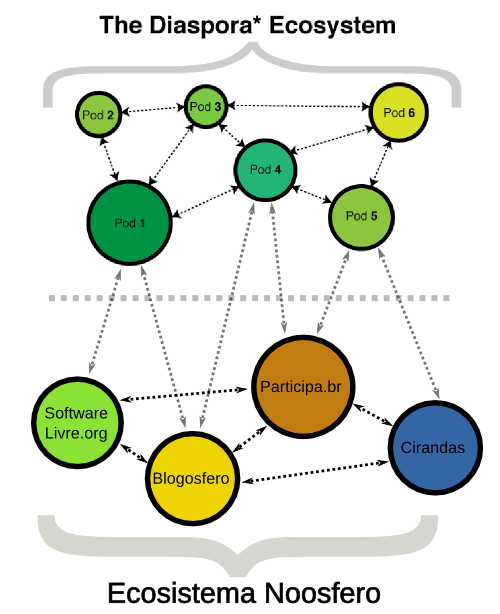
\includegraphics[scale=0.4]{ecosistema-noosfero-diaspora-v2.png}
\caption{Diagrama sobre integração entre redes Noosfero entre sí}
\label{ecosistema-v2}
\end{figure}

A partir da implementação dos protocolos citados acima, o Noosfero ganha
também a capacidade de interagir de forma federada entre sí, ou seja, redes
distintas usando o Noosfero poderão se comunicar de forma transparente através
dos protocolos implementados, um diagrama na Figura \ref{ecosistema-v2}
demonstra essa integração entre redes Noosfero.

\section{Federação entre o Participa.br e redes sociais proprietárias}

Foi desenvolvido no Noosfero através da parceiria entre SG/PR e Serpro um
plugin para adicionar suporte a login via Google e Facebook através do
protocolo OAuth, com isto o Participa.br atualmente já integra com estas duas
redes proprietárias possibilitando seus usuários iniciar sessão através de
seus usuários Google ou Facebook.

O desenvolvimento e o código fonte desta funcionalidade estão documentados nos
links abaixo:

\begin{itemize}
  \item https://gitlab.com/participa/noosfero/issues/186
  \item https://gitlab.com/participa/noosfero/tree/oauth\_rails3
\end{itemize}

%Outra iniciativa em paralelo para oauth também foi desenvolvida aqui:
%https://gitlab.com/noosfero/noosfero/merge\_requests/342

\section{Conclusão}

Neste documento foi apresentado um \ProductDescription

Na prática, este conjunto de informações irá possibilitar aos usuários do
Participa.br se relacionar com usuários de outras redes sociais usamdo o
protocolo Diaspora, além de proporcionar esta mesma capacidade entre usuários
de outras redes usando o Noosfero. Ou seja, um certo usuário do Participa.br
poderá enviar e receber notificações para um usuário localizado na rede {\it
Diaspora* Brazil}\footnote{https://diasporabrazil.org}, ou mesmo na rede {\it
nerdpol.ch Diaspora*}\footnote{https://nerdpol.ch}, ou qualquer outra rede
Diaspora*. Será possível ainda que usuários do Participa.br se relacionem com
usuários de outras redes Noosfero, como por exemplo: SoftwareLivre.org,
Blogoosfero, Cirandas.net, entre outras.

Lembramos que para tornar o Portal de Consulta Pública realmente um canal de
consulta e participação popular na discussão e na definição da agenda
prioritária do país, é necessário que além de documentação faça-se um esforço
de movimentar as pessoar fora do ambiente virtual, para que haja um
engajamento no uso e contribuição deste projeto de forma consistente e perene.

\newpage
\bibliography{bibliografia}
\newpage
\listoffigures
\newpage
\printindex

\end{document}
